\chapter[Introdução]{Introdução}

Esse capítulo apresenta o problema que o trabalho busca solucionar através dos objetivos também apresentados nesse capítulo.

\section{Problema}

Durante o desenvolvimento de um projeto da organização alvo deste trabalho, foi percebido que estavam ocorrendo muitos
atrasos. Considerando as características dos projetos da organização (seção \ref{organizacao}), como o prazo fixo
esses atrasos trazem grandes prejuízos ao escopo e finalização do trabalho. Assim a questão de pesquisa deste trabalho é:

\begin{centering}
 \textit{Como evitar os atrasos nas sprints entendendo os fatores que os influenciam?}.
\end{centering}

\vfill
\pagebreak
  
\section{Objetivos}

	Nesta seção são apresentados os objetivos, geral e específicos, do trabalho definidos a fim de responder a questão de pesquisa definida.

\subsection{Objetivo Geral}

\begin{itemize}
  \item Evitar os atrasos nas sprints mitigando os fatores que os causam.
\end{itemize}

\subsection{Objetivos Específicos}

\begin{itemize}
  \item Conhecer os fatores que influenciam os atrasos em um projeto da organização;
  \item Propor uma estratégia de melhoria a partir dos fatores identificados;
  \item Propor um plano de medição para apoiar essa estratégia;
  \item Avaliar a estratégia definida.
\end{itemize}

\vfill
\pagebreak

\section{Materiais e métodos}

Para este trabalho primeiramente foi realizada uma revisão de literatura simples
para conhecer mais sobre o assunto tratado, observando pesquisas com problemas semelhantes e
as soluções obtidas.

Como metodologia principal foi utilizada uma pesquisa-ação tendo como objeto de estudo um projeto de uma organização descrita no capítulo \ref{pesquisa_acao}. A pesquisa-ação realizada foi composta das fases representadas na Figura \ref{fig:metodologia}.


\begin{figure}[!htb]
\centering
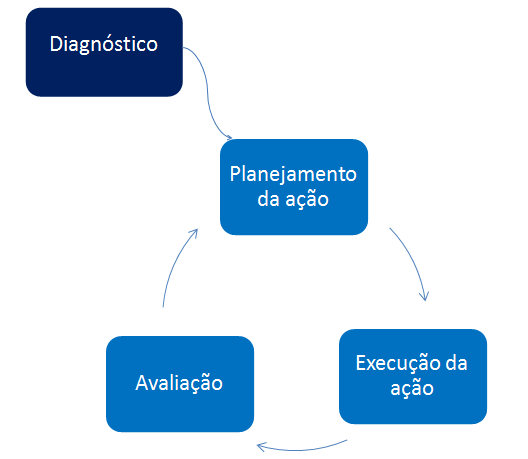
\includegraphics[scale=1]{figuras/pesquisaacao.png}
\caption{Fases da pesquisa-ação. Baseado em \cite{artigo_pesquisa_acao}}
\label{fig:metodologia}
\end{figure}

\pagebreak

De acordo com \citeonline{artigo_pesquisa_acao}, uma pesquisa-ação é composta das seguintes fases:
	\begin{itemize}
		\item \textbf{Diagnóstico:} Essa fase tem como objetivo principal conhecer a situação atual e o problema relacionado ao objeto de estudo. Para realização do diagnóstico foram aplicados questionários.
		\item \textbf{Planejamento da ação:} Essa fase tem como objetivo propor uma ação para resolver o problema diagnosticado, definindo o número de ciclos, as atividades da ação, os envolvidos e como a ação será avaliada.
		\item \textbf{Execução da ação:} Essa fase consiste em executar a ação proposta e acompanhá-la.
		\item \textbf{Avaliação da ação:} Essa fase consiste na avaliação da ação executada a fim de realizar melhorias no próximo ciclo para a ação proposta.
	\end{itemize}

